\documentclass[twoside,10pt]{article}
\usepackage{amsmath,amsfonts,amsthm,fullpage}
\usepackage{mymath}
\usepackage{algorithm}
\usepackage{algorithmic}
\usepackage{graphicx}
\usepackage{mathtools}
\usepackage{hyperref}


\begin{document}

\title{CS 7641 CSE/ISYE 6740 Homework 1}
\author{Rakesh Surapaneni}
\maketitle
\section{Probability [15 pts]}
\subsubsection*{(a) Stores A, B, and C have 50, 75, and 100 employees and, respectively, 50, 60, and 70 percent of these are women. Resignations are equally likely among all employees, regardless of stores and sex. Suppose an employee resigned, and this was a woman. What is the probability that she has worked in store C? [5 pts]}

\textbf{ Solution: }
    Assumptions and definitions: \\
\begin{itemize}
    \item Let W denote the event that the person resigning is a Woman. P(W) is probability that a woman resigns. \\
    \item Let 'a' denotes an event that Store A employee resigns. Similarly events 'b' and 'c' are defined.
    \item P(W/a) = 0.5 (since there are 50\% of employees in store A is Woman and resignations are equally likely irrespective of stores and sex).
    \item Similarly P(W/b) = 0.6 and P(W/c) = 0.7
    \item $$P(a) = \frac{50}{50+75+100} = \frac{50}{225}$$
    \item Similarly P(b) = 75/225, P(c) = 100/225
\end{itemize}
We have to calculate P(c/W) (Probability that store C employee resigns given a Woman resigns)\\
\begin{equation} \nonumber
P(W) = \sum_{x = a,b,c}^{} P(W/x)P(x)\\
= P(W/a)*P(a) + P(W/b)*P(b) + P(W/c)*P(c)\\
= \frac{0.5*50+0.6*75+0.7*100}{225} \\
= \frac{140}{225}
\end{equation}
\begin{equation} \nonumber
P(c/W) = \frac{P(W/c)P(c)}{P(W)}\\
=\frac{0.7*\frac{100}{225}}{\frac{140}{225}}\\
= \frac{70}{140}\\
= 0.5
\end{equation}
Hence if an employee resigned, and this was a woman, the probability that she has worked in store C is \textbf{0.5}.


\vspace{1cm}


\subsubsection*{(b) A laboratory blood test is 95 percent effective in detecting a certain disease when it is, in fact, present. The test also yields a false positive result for 1 percent of the healthy persons tested. That is, if a healthy person is tested then with probability 0.01 the test result will imply he has the disease. If 0.5 percent of the population actually has the disease, what is the probability a person has the disease given that his test result is positive? [5 pts]}

\textbf{ Solution: }	
 Assumptions and definitions: \\
\begin{itemize}
    \item Let x denote the event that the result is positive. 
    \item y denote the event that the result is negative.
    \item D denote the event that there is disease and N denotes that there is no disease.
    \item We are given that P(x/D) = 0.95 (accuracy in case of disease).
    \item P(x/N) = 0.01 (false positives).
    \item P(D) = 0.005 P(N) = 0.995 (0.5\% have the disease).
    \item We have to find \textbf{P(D/x)}.
\end{itemize}
\begin{equation*}
P(x) = P(x and D) + P(x and N)
\end{equation*}
\begin{equation*}
= P(D)*P(x/D) + P(N)* P(x/N)
\end{equation*}
\begin{equation*}
=0.005*0.95 + 0.995*0.01 
\end{equation*}
\begin{equation*}\label{eq1}
P(x) = 0.0147
\end{equation*}
\begin{equation*}
p(D/x) = \frac{P(x/D)P(D)}{P(x)} -- By Bayes Theorem
\end{equation*}
\begin{equation*}
= \frac{0.95*0.005}{0.0147} -- By using \ref{eq1}
\end{equation*}
\begin{equation*}
= \frac{0.475}{1.47} = 0.3231292517
\end{equation*}
Hence probability a person has the disease given that his test result is positive is \textbf{0.3231292517}.


%page for c
%\newpage
\vspace{1cm}



\textbf{[c-d]} On the morning of September 31, 1982, the won-lost records of the three leading baseball teams in the western division of the National League of the United States were as follows:

\begin{table}[!h]
\centering \small
\begin{tabular}{l|c|c}
  \hline
  Team & Won & Lost\\
  \hline \hline
  Atlanta Braves & 87 & 72\\
  San Francisco Giants & 86 & 73\\
  Los Angeles Dodgers & 86 & 73\\
  \hline
\end{tabular}
\end{table}

Each team had 3 games remaining to be played. All 3 of the Giants games were with the Dodgers, and the 3 remaining games of the Braves were against the San Diego Padres. Suppose that the outcomes of all remaining games are independent and each game is equally likely to be won by either participant. If two teams tie for first place, they have a playoff game, which each team has an equal chance of winning.


\vspace{1cm}

\subsubsection*{(c) What is the probability that Atlanta Braves wins the division? [2 pts]}
\textbf{ Solution: }	
There are four possible cases when Atlanta Braves can win the division.
\begin{itemize}
	\item \textbf{case 1:} (Event C1) Braves wins all three games with Padres.\\
   	\begin{equation*}\label{c1}
		P(C1) = 1/2*1/2*1/2 = 1/8 
	\end{equation*}
    \item \textbf{case 2:} (Event C2) Braves wins two out of three games . If either Giants or dodgers win three games(1/8 probability each), it leads to additional playoff. Then Braves win with probability 1/2 in playoff.
    P(C2) = Prob of braves winning playoff(1/2) * prob of giant or dodgers winning 3 games(1/8+ 1/8)* prob of braves winning 2 games in initial set(3/8 (3 possibilities 1/8 each))
   	\begin{equation*}\label{c2}
		P(C2) =  1/2*(2/8)*3/8 = 3/64
	\end{equation*}
    \item \textbf{case 3:} (Event C3) Braves wins two out of three games(3/8) and giant or dodgers wins only 2 games(3/8+3/8). There is no need for playoff since braves are already leading.
   	\begin{equation*}\label{c3}
		P(C3) =  3/8*3/4 = 9/32
	\end{equation*}
     \item \textbf{case 4:} (Event C4)  Braves wins one out of three games(3/8) and giant or dodgers wins only 2 games(3/8+3/8), it leads to additional playoff. Then Braves win with probability 1/2 in playoff.
   	\begin{equation*}\label{c4}
		P(C4) =  1/2*(6/8)*3/8 = 9/64
	\end{equation*}
\end{itemize}
Probability of Braves winning the tournament = (1/8+3/64 + 9/32 + 9/64)\\
= \textbf{0.59375}


%page for d
%\newpage
\vspace{1cm}

\subsubsection*{(d) What is the probability to have an additional playoff game? [3 pts]}
\textbf{ Solution: }	
Assuming that Padres are not good enough to enter playoffs, the only teams that can compete in playoff are Atlanta Braves vs either giants or dodgers. \\(There is no possibility of payoffs b/n giants and Dogers since they are at equal points and they have odd number of games b/n them.)\\
Following are the cases when Braves and giants/dodgers can enter playoffs
\begin{itemize}
\item \textbf{case 1:} (Event C1) ATL Braves wins 2 games(3/8) and either Dodgers or Giants wins 3 games(1/8+1/8) (P(C1) = 3/32)
\item \textbf{case 2:} (Event C2) ATL Braves wins 1 games(3/8) and neigher dodgers or giants win three games (3/4) P(C2 = 9/32)
\end{itemize}
Overall probability of playoff = 3/32+9/32 = 12/32 = 0.375\\
Hence probability to have an additional playoff game is \textbf{0.375}
%\vspace{1cm}
\newpage

%----------------------------------------------------------------------------------
\section{Maximum Likelihood [15 pts]}

Suppose we have $n$ i.i.d (independent and identically distributed)
data samples from the following probability distribution. This
problem asks you to build a log-likelihood function, and find the
maximum likelihood estimator of the parameter(s).

\subsubsection*{(a) Poisson distribution [5 pts]}
The Poisson distribution is defined as
\begin{equation} \nonumber
P(x_i = k) = \frac{\lambda^k e^{-\lambda}}{k!} (k = 0, 1, 2, ...).
\end{equation}
What is the maximum likelihood estimator of $\lambda$?
\textbf{Solution:}

\begin{equation} \nonumber
P(x_i = k) = \frac{\lambda^k e^{-\lambda}}{k!} (k = 0, 1, 2, ...).
\end{equation}
We have n total number of values for k.\\
Log likelihood estimator function 
\begin{equation} \nonumber
L(sample/\lambda) = Log(\prod_{k = 0}^{n-1}{P(x_i = k)}) (k = 0, 1, 2, ...).
\end{equation}
\begin{equation} \nonumber
= Log(\prod_{i = 0}^{n-1}{\frac{\lambda^x_i e^{-\lambda}}{x_i!}}) 
\end{equation}
\begin{equation} \nonumber
= \sum_{i = 0}^{n-1} { Log({\frac{\lambda^x_i e^{-\lambda}}{x_i!}}) }
\end{equation}
\begin{equation} \nonumber
= \sum_{k = 0}^{n-1} { (x_i(Log(\lambda))-\lambda+log(x_i!) )}
\end{equation}

The arg max at which the log-likelihood is maximized, derivative is 0. 
\begin{equation} \nonumber
\frac{\partial L}{\partial \lambda}= \sum_{k = 0}^{n-1} { \frac{x_i}{\lambda}-1 } = 0
\end{equation}
\begin{equation} \nonumber
=> \sum_{i = 0}^{n-1} { \frac{x_i}{\lambda}-1 } = 0
\end{equation}
\begin{equation} \nonumber
=> \lambda = \sum_{i = 0}^{n-1} { x_i }/n 
\end{equation}

Hence maximum likelihood estimation of $\lambda$ is 
\begin{equation} \nonumber
\boxed{\lambda = \sum_{i = 0}^{n-1} { x_i }/n }
\end{equation}


\vspace{1cm}
\subsubsection*{(b) Multinomial distribution [5 pts]}
The probability density function of Multinomial distribution is given by 
$$f(x_1,x_2,\dots,x_k;n,\theta_1,\theta_2,\dots,\theta_k)=\frac{n!}{x_1!x_2!\cdots x_k!}\prod_{j=1}^{k}\theta_j^{x_j},$$
where $\sum_{j=1}^k\theta_j=1,\sum_{j=1}^k x_j=n$. What is the maximum likelihood estimator of $\theta_j, j=1,\dots k$?\\
  
\textbf{Solution:}
$$f(x_1,x_2,\dots,x_k;n,\theta_1,\theta_2,\dots,\theta_k)=\frac{n!}{x_1!x_2!\cdots x_k!}\prod_{j=1}^{k}\theta_j^{x_j},$$
\begin{equation} \nonumber
=> L = log(f) = log(\frac{n!}{x_1!x_2!\cdots x_k!}\prod_{j=1}^{k}\theta_j^{x_j})
\end{equation}
\begin{equation} \label{2b1}
= log(\frac{n!}{x_1!x_2!\cdots x_k!}) + \sum_{j=1}^{k}{x_j}log{\theta_j}
\end{equation}
We know that 
\begin{equation} \nonumber
\sum_{j=1}^{k}{x_j} = n 
\end{equation}
\begin{equation} \label{xsum}
=> x_k = n - \sum_{j=1}^{k-1}{x_j}\&\&
\end{equation}
\begin{equation} \nonumber
\sum_{j=1}^{k}{\theta_j} = 1 
\end{equation}
\begin{equation} \label{tsum}
=> theta_k = 1 - \sum_{j=1}^{k-1}{\theta_j}
\end{equation}

from \label{2b1}, \label{xsum} and \label{tsum}, we can say that 
\begin{equation} \nonumber
L = log(\frac{n!}{x_1!x_2!\cdots x_k!}) + \sum_{j=1}^{k-1}{x_j}log{\theta_j}
+ {x_k}log(1-\sum_{j=1}^{k-1}{\theta_j})
\end{equation}
At arg max L
\begin{equation} \nonumber
\frac{\partial L}{\partial \theta_j} = 0 for all j from 1 to k-1
\end{equation}
(Note that last theta depends on other values and hence not an independent variable)
\begin{equation} \nonumber
=> \frac{x_j}{\theta_j}
-\frac{x_k}{1-\sum_{j=1}^{k-1}{\theta_j}} = 0
\end{equation}
\begin{equation} \nonumber
=> \frac{x_j}{\theta_j}
-\frac{x_k}{\theta_k} = 0 
\end{equation}
for all j = 1,2,3,4...k-1\\
Let
\begin{equation} \nonumber
=> \frac{x_j}{\theta_j} = c
\end{equation}
\begin{equation} \nonumber
=> x_j = c*{\theta_j}
\end{equation}
summing and applying \label{xsum} and \label{tsum}
\begin{equation} \nonumber
=> \sum{x_j} = c*{sum{\theta_j}}
\end{equation}
\begin{equation} \nonumber
=> c = n
\end{equation}
\textbf{Therefore}
\begin{equation} \nonumber
\theta_j = \frac{x_j}{n}
\end{equation}

\vspace{1cm}

\subsubsection*{(c) Gaussian normal distribution [5 pts]}
Suppose we have $n$ i.i.d (Independent and Identically Distributed)
data samples from a univariate Gaussian normal distribution
$\mathcal{N}(\mu, \sigma^2)$, which is given by
\begin{equation}
\mathcal{N}(x; \mu, \sigma^2) = \frac{1}{\sigma \sqrt{2\pi}} \exp
\left( - \frac{(x - \mu)^2}{2\sigma^2} \right).\nonumber
\end{equation}
What is the maximum likelihood estimator of $\mu$ and $\sigma^2$?

\textbf{Solution:}
Let $$x_1,x_2,...x_n$$ be the n samples which are observed.
log Likelihood function:
\begin{equation}\nonumber
L = log\prod_{j=1}^{k}{\frac{1}{\sigma \sqrt{2\pi}}}\exp
\left( - \frac{(x_j - \mu)^2}{2\sigma^2} \right).
\end{equation}
\begin{equation}\nonumber
= n*log{\frac{1}{\sigma \sqrt{2\pi}}} - \sum_{j = 1}^{n}\frac{(x_j - \mu)^2}{2\sigma^2} .
\end{equation}
\begin{equation}\nonumber
= n/2*log{\frac{1}{\sigma^2 2\pi}} - \sum_{j = 1}^{n}\frac{(x_j  - \mu)^2}{2\sigma^2} .
\end{equation}
To maximising L using $$\mu$$ we get
\begin{equation}\nonumber
\frac{\partial L}{\partial \mu}= 0
\end{equation}
\begin{equation}\nonumber
=>\sum_{j = 1}^{n}\frac{-2(x_j - \mu)}{2\sigma^2}= 0
\end{equation}
\begin{equation}\nonumber
=>\sum_{j = 1}^{n}\frac{-2(x_j - \mu)}{2\sigma^2}= 0
\end{equation}
\begin{equation}\nonumber
=>\sum_{j = 1}^{n}\frac{-2(x_j - \mu)} = 0
\end{equation}
\begin{equation}\nonumber
=>\mu = \frac{\sum_{j=1}^{n}x_j}{n} --> \textbf{Answer}
\end{equation}
To maximise L using $$\sigma^2$$ we get
\begin{equation}\nonumber
\frac{\partial L}{\partial \sigma^2}= 0
\end{equation}
\begin{equation}\nonumber
=> \sum_{j = 1}^{k}{-\frac{-(x_j-\mu)^2}{2\sigma^4}} - n/2*\frac{\sigma^2 2\pi}{{\sigma^2}^2 2\pi}= 0
\end{equation}
\begin{equation}\nonumber
=> \sum_{j = 1}^{k}{\frac{(x_j-\mu)^2}{2\sigma^2}} - n/2= 0
\end{equation}
\begin{equation}\nonumber
=> \sigma^2 = \sum_{j = 1}^{k}{\frac{(x_j-\mu)^2}{n}} -- \textbf{Answer}
\end{equation}
\vspace{1cm}

\iffalse
\subsubsection*{(b) Exponential distribution [5 pts]}
The probability density function of Exponential distribution is
given by
\begin{equation} \nonumber
f(x) = \left\{\begin{matrix}
\lambda e^{-\lambda x} & x \ge 0\\
0 & x < 0
\end{matrix}\right.
\end{equation}
What is the maximum likelihood estimator of $\lambda$?
\fi
\newpage
%----------------------------------------------------------------------------------
\section{Principal Component Analysis [20 pts]}
In class, we learned that Principal Component Analysis (PCA)
preserves variance as much as possible. We are going to explore
another way of deriving it: minimizing reconstruction error.

Consider data points $\text x^n (n=1, ..., N)$ in $D$-dimensional space.
We are going to represent them in $\{\text u_1, ..., \text u_D\}$ orthonormal basis.
That is,
\begin{equation} \nonumber
\text x^n = \sum_{i=1}^D \alpha_i^n \text u_i = \sum_{i=1}^D ({\text x^n}^T \text u_i) \text u_i.
\end{equation}
Here, $\alpha^n_i$ is the length when $\text x^n$ is projected onto
$u_i$.

Suppose we want to reduce the dimension from $D$ to $M < D$. Then
the data point $\text x^n$ is approximated by
\begin{equation} \nonumber
\tilde{\text x}^n = \sum_{i=1}^M z_i^n \text u_i + \sum_{i=M+1}^D b_i \text u_i.
\end{equation}
In this representation, the first $M$ directions of $\text u_i$ are
allowed to have different coefficient $z^n_i$ for each data point,
while the rest has a constant coefficient $b_i$. As long as it is
the same value for all data points, it does not need to be 0.

Our goal is setting $\text u_i$, $z^n_i$, and $b_i$ for $n = 1,..., N$
and $i = 1, ..., D$ so as to minimize reconstruction error. That is,
we want to minimize the difference between $\text x^n$ and $\tilde{\text x}^n$ over $\{ \text u_i, z^n_i, b_i \}$:
\begin{equation} \nonumber
J = \frac{1}{N} \sum_{n=1}^N \| \text x^n - \tilde{\text x}^n \|^2.
\end{equation}

\subsubsection*{(a) What is the assignment of $z_j^n$ for $j=1, ..., M$ minimizing $J$? [5 pts]}
\textbf{Solution:}\\
$$J = \frac{1}{N} \sum_{n=1}^N \| \text x^n - \tilde{\text x}^n \|^2. $$
Since all $u_i$'s are Ortho-normal to each other,$u_i u_j = 0$ for all i!= j
Hence by expanding J we get
$$J = \frac{1}{N} \sum_{n=1}^N ( \text x^n - \tilde{\text x}^n )^T ( \text x^n - \tilde{\text x}^n ). $$
$$  = \frac{1}{N} \sum_{n=1}^N{(\sum_{i=1}^M{(\alpha_i^n - z_i^n)u_i} + \sum_{i=M+1}^D{(\alpha_i^n - b_i)u_i})^T(\sum_{i=1}^M{(\alpha_i^n - z_i^n)u_i} + \sum_{i=M+1}^D{(\alpha_i^n - b_i)u_i})}$$
\begin{equation}\label{eq_4}
J  = \frac{1}{N} \sum_{n=1}^N{\sum_{i=1}^M{(\alpha_i^n - z_i^n)^2u_i^T u_i} + \sum_{i=M+1}^D{(\alpha_i^n - b_i)^2u_i^T u_i}}
\end{equation}
(since cross multiplication terms where $u_i$ and $u_j$ are multiplied are 0 due to ortho-normal property)\\
\hspace{1cm}
To minimize J w.r.t $z_j^n$ , we differential and make it 0 for all the n and j values.
$$\frac{\partial J}{\partial z_j^n} = \frac{1}{N}2(\alpha_i^n - z_i^n)(-1) = 0$$
$$=> \boxed{z_i^n = \alpha_i^n} --> \textbf{Answer} $$
$$=> \boxed{z_i^n = x^{n^T}u_i} --> \textbf{Answer} $$


\subsubsection*{(b) What is the assignment of $b_j$ for $j=M+1, ..., D$ minimizing $J$? [5 pts]}
\textbf{Answer:}\\
By using equation \ref{eq_4}, we know that 
$$J  = \frac{1}{N} \sum_{n=1}^N{\sum_{i=1}^M{(\alpha_i^n - z_i^n)^2u_i^T u_i} + \sum_{i=M+1}^D{(\alpha_i^n - b_i)^2u_i^T u_i}}$$
To find $b_j$ that minimizes J,
$$\frac{\partial J}{\partial b_j} = \frac{1}{N}\sum_{n=1}^N{2(\alpha_j^n - b_j)} = 0 $$
$$=> \frac{1}{N}\sum_{n=1}^N{2(\alpha_j^n - b_j)} = 0 $$
$$=> \sum_{n=1}^N{(\alpha_j^n)} = \sum_{n=1}^N{(b_j)}  $$
$$=> \sum_{n=1}^N{(\alpha_j^n)} = N*b_j  $$
$$=> \boxed{b_j = \frac{1}{N}\sum_{n=1}^N{(\alpha_j^n)}}  $$
$$=> \boxed{b_j = \frac{1}{N}\sum_{n=1}^N{(x^{n^T}u_j)}}  -->\textbf{Answer}$$



\subsubsection*{(c) Express optimal $\tilde{\text x}^n$ and $\text x^n - \tilde{\text x}^n$ using your answer for (a) and (b). [2 pts]}
By using equation \ref{eq_4} and results from above, we know 
$$\tilde{\text x}^n = \sum_{i=1}^M{z_i^nu_i} + \sum_{i=M+1}^D{b_iu_i}$$
$$\boxed{\tilde{\text x}^n = \sum_{i=1}^M{(x^{n^T}u_i)u_i} + \sum_{i=M+1}^D{\mu_iu_i}}$$
where $\mu_i$ = mean of all $x_i^n$'s. 
$$\text x^n - \tilde{\text x}^n = \sum_{i=1}^M{(x^{n^T}u_i)u_i - (x^{n^T}u_i)u_i} + \sum_{i=M+1}^D{(x^{n^T}u_i)u_i - \mu_iu_i}$$
$$\boxed{\text x^n - \tilde{\text x}^n = \sum_{i=M+1}^D{(x^{n^T}u_i)u_i - \bar{\text x_i}u_i}}$$

\subsubsection*{(d) What should be the $\text u_i$ for $i=1, ..., D$ to minimize $J$? [8 pts]}
\emph{Hint:} Use $S = \frac{1}{N} \sum_{n=1}^N (\text x^n - \bar{\text x})(\text x^n -
\bar{\text x})^T$ for sample co-variance matrix. \vspace{1cm}

\textbf{Ans:}\\
We know that S is co-variance matrix. 
$$u_j^TSu_j = \frac{1}{N} \sum_{n=1}^N {u_j^T(x^n-\tilde{\text x})(x^n-\tilde{\text x})^Tu_j}$$
The above equation is square of "projection of $x^n-\tilde{\text x}$ on top of $u_j$".

$$\sum_{j = 1}^D u_j^TSu_j = \frac{1}{N} \sum_{j = 1}^D \sum_{n=1}^N {u_j^T(x^n-\tilde{\text x})(x^n-\tilde{\text x})^Tu_j}$$
$$ = \frac{1}{N} \sum_{n=1}^N \| \text x^n - \tilde{\text x}^n \|^2.$$
We know that $u_j^Tu_j = 1$ for all j's due to the ortho-normal property.
Hence we can add Lagrange term just like in PCA derivation as follows

$$J = \frac{1}{N} \sum_{n=1}^N \| \text x^n - \tilde{\text x}^n \|^2 + \lambda (D - \sum_{j = 1}^D{u_i^Tu_i})$$
$$J = \sum_{j=1}^D{u_j^TSu_j} + \lambda (D - \sum_{j = 1}^D{u_i^Tu_i})$$
$$J = \sum_{j=1}^D{u_j^TSu_j+\lambda (1 - u_i^Tu_i)}$$
To maximize J w.r.t $u_i$, we take derivative.

$$\frac{\partial J}{\partial u_i} = {u_i^TSu_i\lambda ( - 2u_i^T)}$$
Source: \href{https://en.wikipedia.org/wiki/Matrix_calculus}{wiki page for matrix calculus} \\
I have checked differentiating $x^Tx$ gives $2x^T$.
Now this equation is similar to one we have solved in PCA. applying same reduction we get u's being \textbf{Eigen-vectors} of S. TO minimize J, we pick D eigen vectors in decreasing order of their Eigen-values. first M values have M highest eigen values.
\newpage
%----------------------------------------------------------------------------------
\section{Clustering [20 pts]}

\textbf{[a-b]} Given $N$ data points $\text x^n (n=1,\dots,N)$, $K$-means clustering algorithm groups them into $K$ clusters by minimizing the distortion function over $\{ r^{nk}, \mu^k \}$
$$J=\sum_{n=1}^N\sum_{k=1}^Kr^{nk} \|\text x^n-\mu^k\|^2,$$
where $r^{nk}=1$ if $\text x^n$ belongs to the $k$-th cluster and $r^{nk}=0$ otherwise.

\subsubsection*{(a) Prove that using the squared Euclidean distance $\|\text x^n-\mu^k\|^2$ as the dissimilarity function and minimizing the distortion function, we will have 
   $$\mu^k=\frac{\sum_n r^{nk} \text x_n}{\sum_n r^{nk}}.$$
   That is, $\mu^k$ is the center of $k$-th cluster. [5 pts]}
\textbf{solution}: 
Given that 
$$J=\sum_{n=1}^N\sum_{k=1}^Kr^{nk} \|\text x^n-\mu^k\|^2,$$
Clearly J is at an optima when 
$$\frac{\partial J}{\partial \mu^i} = 0$$
$$=>\frac{\partial \sum_{n=1}^N\sum_{k=1}^Kr^{nk} \|\text x^n-\mu^k\|^2}{\partial \mu^i} = 0$$
$$=>\sum_{n=1}^N{2r^{ni}}*(x^n-\mu^i) = 0$$
$$=> \mu^i = \frac{\sum_{n=1}^N{r^{ni}x^n}}{\sum_{n=1}^N{r^{ni}}}$$

\hspace{1cm} To prove that this point which is an optima is infact a argmin is by taking very large values of $\mu$. J values for large $\mu$ is very high which indicates that this point is a minimum where cost 'J' is minimized.\\
\hspace{1cm} \textbf{Hence} minimizing the distortion function 'J', we get 
$$\mu^k=\frac{\sum_n r^{nk} \text x_n}{\sum_n r^{nk}}.$$
\subsubsection*{(b) Prove that $K$-means algorithm converges to a local optimum in finite steps. [5 pts]}
\begin{itemize}
\item If in any step of iteration, if the J value doesn't decrease, then we have already converged to a local minima.
\item There are $k^n$ possible cluster assignments (each point can be assigned to one of k clusters). In each cluster assignment there can be unique minima as shown in part 1 where center is taken as the argmin
\item also in each iteration, we change cluster assignment only if the cost decreases. Recaculating the cluster center will further reduce the 'J' value.
\item Hence using above argument since there are finite possible cost values and in each iterations cost decreases, it will eventually reach Minima where we define algorithm to converge.
\end{itemize}

\textbf{[c-d]} In class, we discussed bottom-up hierarchical clustering. For each iteration, we need to find two clusters $\{\text x_1, \text x_2, \dots, \text x_m\}$ and $\{\text y_1, \text y_2, \dots, \text y_p\}$ with the minimum distance to merge. Some of the most commonly used distance metrics between two clusters are:
    \begin{itemize}
    \item Single linkage: the minimum distance between any pairs of points from the two clusters, i.e.
    $$\min_{i=1,\dots,m \atop j=1,\dots, p}\|\text x_i - \text y_j\|$$
    \item Complete linkage: the maximum distance between any parts of points from the two clusters, i.e.
    $$\max_{i=1,\dots,m \atop j=1,\dots, p}\|\text x_i - \text y_j\|$$
    \item Average linkage: the average distance between all pair of points from the two clusters, i.e.
    $$\frac{1}{mp}\sum_{i=1}^m\sum_{j=1}^p\|\text x_i - \text y_j\|$$
    \end{itemize}

\subsubsection*{(c) When we use the bottom up hierarchical clustering to realize the partition of data, which of the three cluster distance metrics described above would most likely result in clusters most similar to those given by $K$-means? (Suppose $K$ is a power of 2 in this case). [5 pts]}

\textbf{Solution:}
\hspace{1cm} The average linkage is very the best strategy here. Note that k-means and average linkage both uses the means as a base of deciding connectivity. Hence Average linkage is the best metric here.
\subsubsection*{(d) For the following data (two moons), which of these three distance metrics (if any) would successfully separate the two moons? [5 pts]}

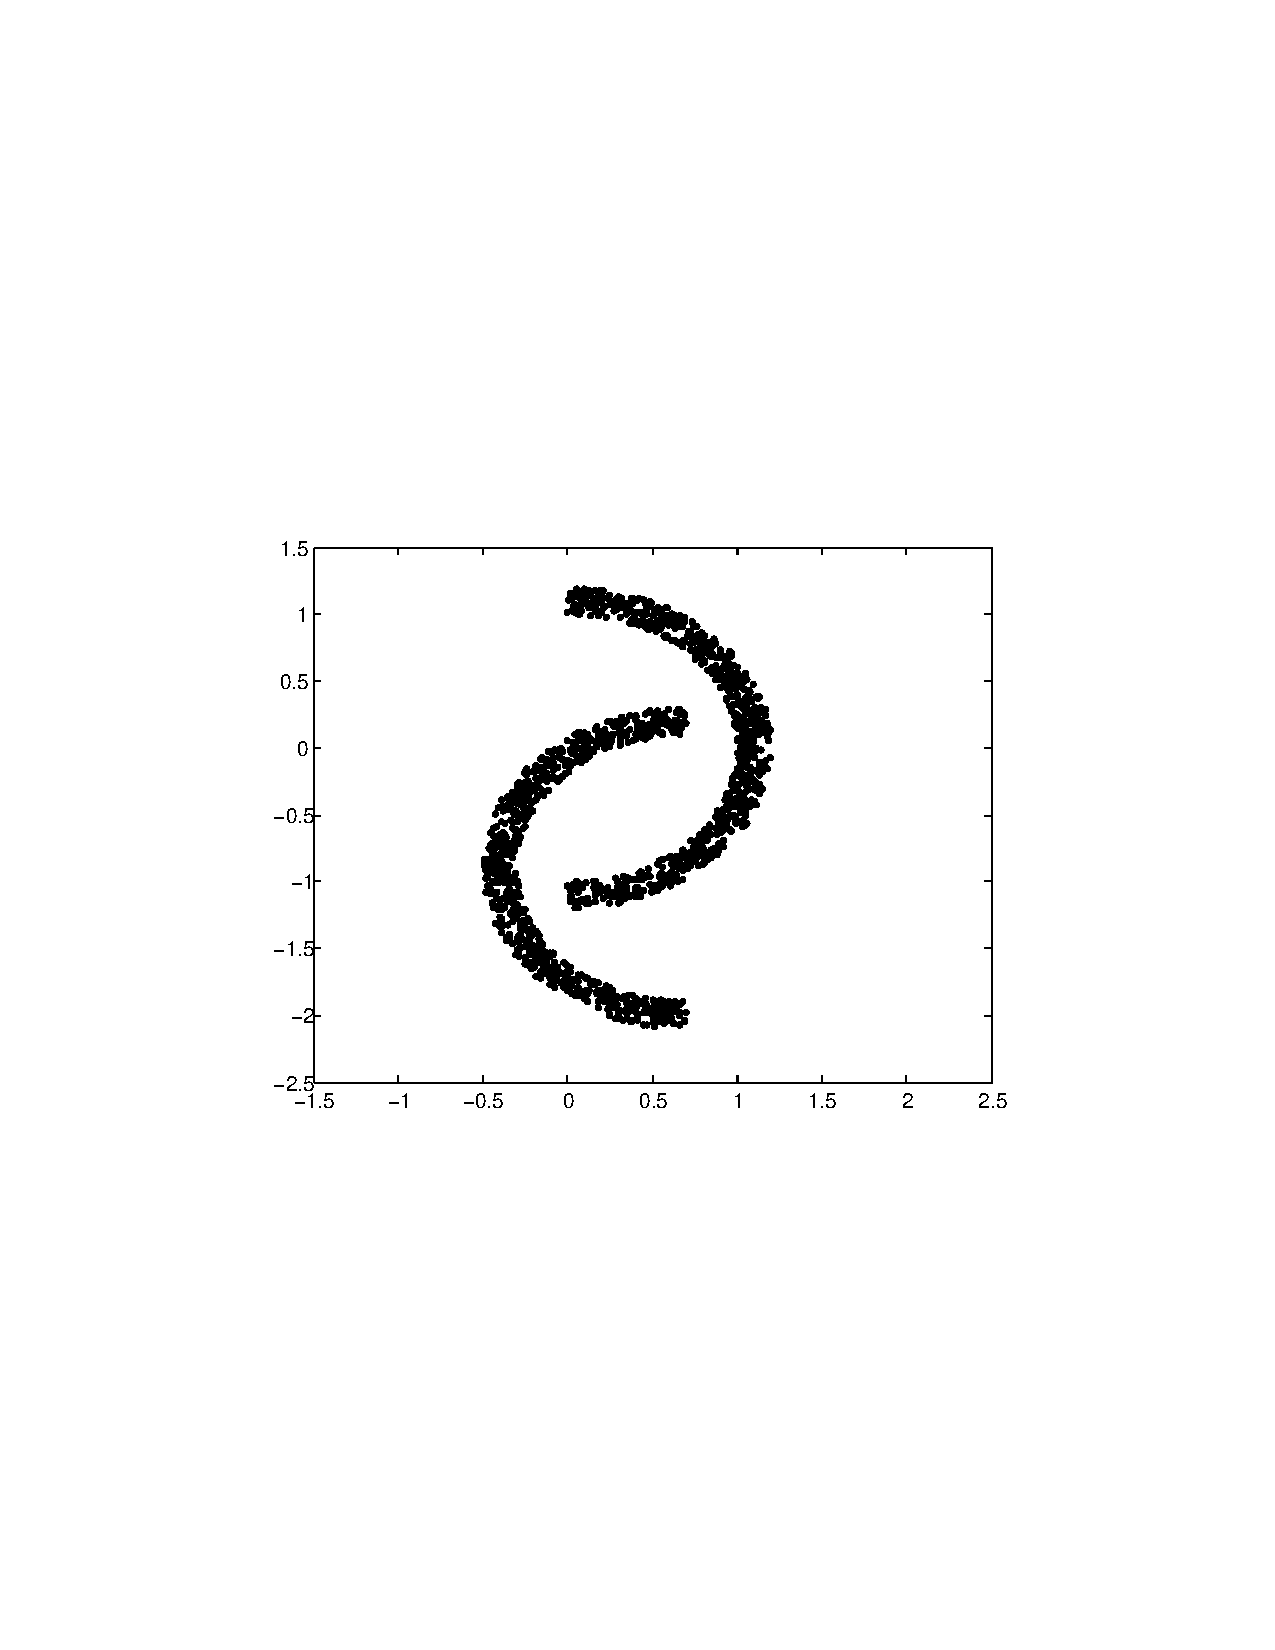
\includegraphics[trim = 0mm 90mm 0mm 90mm, clip, width = \linewidth]{clustering}

\textbf{Solution:}
\begin{itemize}
\item Single Linkage is the best algorithm to use here. Spectral clustering is the best algorithm to use in this scenario and spectral clustering is essentially uses same ideology.
\item To try to understand this, if we use average of complete linkage, consider scenario where each moons are broken into two halfs. the top half of the left moon is very close to bottom half of right one and they both will be clustered into 1 category. Hence we need to use single linkage.
\end{itemize}
\end{document}



